\documentclass{hwset}

\name{Erich L Foster}
\class{Calculus I}
\duedate{26 April 2011}
\assignment{Homework 12}

\begin{document}
\begin{problem}[1.]
  \tbf{Let's design a can.}
  \begin{enumerate}
    \item A can is to be made to hold volume V. Find the ratio between the
      height $h$ and the radius $r$ that will minimize the cost of the metal to
      manufacture the can, assuming the cost is directly proportional to the
      metal used.
    \item In part (a) we assumed there to be no waste in the making of the can.
      However, in manufacturing the can we must have some waste when creating
      the top and bottom discs. Now assume the top and bottom discs are cut from
      squares as in Figure \ref{fig:squares} and find the ratio of the height
      $h$ to the radius $r$ that minimizes the cost of manufacturing the can.
    \item A more efficient packing of discs can be obtained by diving the metal
      sheet into hexagons and cutting the discs from the hexagons as in Figure
      \ref{fig:hexagons}. If this strategy is adopted find the ratio between the
      height $h$ and the radius $r$ that minimizes the cost of manufacturing the
      can.
  \end{enumerate}
\end{problem}

\begin{enumerate}
  \item \begin{solution}
    The volume of a can is given by
    \begin{equation}
      V = \pi r^2 h
      \label{eqn:CanVol}
    \end{equation}
    From this we find that 
    \begin{equation}
      h = \dfrac{V}{\pi r^2}. 
      \label{eqn:RtoH}
    \end{equation}
    The surface area of a can is
    \begin{align*}
      A &= 2\pi r^2 + 2\pi r h \\
      &= 2\pi r^2 + \frac{2V}{r} .
    \end{align*}
    Since the cost is directly proportional to the material used minimizing the
    amount of material used is equivalent to minimizing the surface area of the
    can. Using the area equation we can determine the critical points
    \begin{align*}
      &\frac{dA}{dr} = 4\pi r - \frac{2V}{r^2} = 0\\
      &\Rightarrow 4\pi r^3 - 2V = 0 \\ 
      &r = \sqrt[3]{\frac{V}{2\pi}} 
    \end{align*}
    The other critical point of $r=0$ comes from when $\dfrac{dA}{dr}$ is
    undefined. However, $r=0$ isn't in the domain of the function, since a can
    with radius zero isn't really a can. Now we must check that
    $r=\sqrt[3]{\dfrac{V}{2\pi}}$ is indeed a minimum. To do this let's use the
    second derivative test
    \begin{align*}
      \left.\frac{d^2A}{dr^2}\right|_{r=\sqrt[3]{\dfrac{V}{2\pi}}} &= 4\pi + \frac{2V}{r^3} \\
      &= 4\pi + \frac{4\pi V}{V} \\
      &= 8\pi.
    \end{align*}
    Since the second derivative at the critical point is positive this is a
    minimum. Therefore, the minimum cost of a can happens when
    \begin{align*}
      r &= \sqrt[3]{\frac{V}{2\pi}} \\
      r &= \sqrt[3]{\frac{\pi r^2 h}{2\pi}} \\
      r^3 &= \frac{r^2 h}{2} \\
      \Rightarrow& \boxed{\sfrac{r}{h}=\sfrac{1}{2}}.
    \end{align*}
  \end{solution}
  \item \begin{solution}
    This time the area equation is given by
    \begin{align*}
      A &= 8r^2 + 2\pi r h \\
      &= 8r^2 + \frac{2v}{r} .
    \end{align*}
    Both equations \eqref{eqn:CanVol} and \eqref{eqn:RtoH} still hold and so to
    find the critical points
    \begin{align*}
      & \dfrac{dA}{dr} = 16 r - \frac{2V}{r^2} = 0 \\
      & \Rightarrow 16 r^3 - 2V = 0 \\
      & r = \sqrt[3]{\frac{V}{8}}.
    \end{align*}
    The other critical point of $r=0$ comes from when $\dfrac{dA}{dr}$ is
    undefined. However, $r=0$ isn't in the domain of the function, since a can
    with radius zero isn't really a can. Now we must check that
    $r=\sqrt[3]{\dfrac{V}{8}}$ is indeed a minimum. To do this let's use the
    second derivative test
    \begin{align*}
      \left.\frac{d^2A}{dr^2}\right|_{r=\sqrt[3]{\dfrac{V}{8}}} &= 16 + \frac{2V}{r^3} \\
      &= 16 + \frac{4\pi V}{V} \\
      &= 16 + 4\pi.
    \end{align*}
    Since the second derivative at the critical point is positive this is a
    minimum. Therefore, the minimum cost of a can happens when
    \begin{align*}
      r &= \sqrt[3]{\frac{V}{8}} \\
      r &= \sqrt[3]{\frac{\pi r^2 h}{8}} \\
      r^3 &= \frac{\pi r^2 h}{8} \\
      \Rightarrow &\boxed{\sfrac{r}{h}=\sfrac{\pi}{8}}.
    \end{align*}
  \end{solution}
  \item \begin{solution}
    The area of a regular hexagon given side $t$ is 
    \begin{equation*}
      A_H = \frac{3\sqrt{3}}{2} t^2
    \end{equation*}
    So first, we must find the relation of a side of the hexagon, $t$, and
    radius of the can, $r$.  Each angle of a hexagon is $120^\circ$ or
    $\sfrac{2\pi}{3}$. Let's form a triangle in the following way
    \begin{center}
    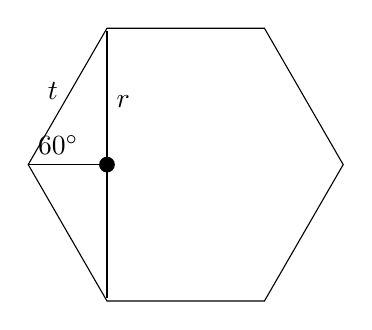
\begin{tikzpicture}
      \def\hex#1#2{
        \draw #1 #2 +(0:2) \foreach \a in {60,120,...,330} { -- +(\a:2) } -- cycle;
      }
      \hex{(0,0)}{(0,0)};
      \draw (-1,1.7) -- (-1,0.8) node[right,fill=none] {$r$} -- (-1,-1.7);
      \draw (-1,0) -- (-2,0) node[above right,fill=none] {$60^\circ$};
      \fill[fill=black] (-1,0) circle(1mm);
      \node at (-1.5,0.7) [above left,fill=none] {$t$}; 
    \end{tikzpicture}
    \end{center}
    Thus, we see
    \begin{align*}
      \sin \frac{\pi}{3} &= \frac{r}{t} \\
      \Rightarrow t &= \frac{2\sqrt{3}}{3} r.
    \end{align*}
    Therefore the area equation is given by
    \begin{align*}
      A &= 3\sqrt{3}\left( \dfrac{2\sqrt{3}}{3} r \right)^2 + 2\pi r h \\
      &= 4\sqrt{3} r^2 + \frac{2v}{r} .
    \end{align*}
    Both equations \eqref{eqn:CanVol} and \eqref{eqn:RtoH} still hold and so to
    find the critical points
    \begin{align*}
      & \dfrac{dA}{dr} = 8\sqrt{3} r - \frac{2V}{r^2} = 0 \\
      & \Rightarrow 8\sqrt{3} r^3 - 2V = 0 \\
      & r = \sqrt[3]{\frac{V}{4\sqrt{3}}}.
    \end{align*}
    The other critical point of $r=0$ comes from when $\dfrac{dA}{dr}$ is
    undefined. However, $r=0$ isn't in the domain of the function, since a can
    with radius zero isn't really a can. Now we must check that
    $r=\sqrt[3]{\dfrac{V}{4\sqrt{3}}}$ is indeed a minimum. To do this let's use the
    second derivative test
    \begin{align*}
      \left.\frac{d^2A}{dr^2}\right|_{r=\sqrt[3]{\dfrac{V}{4\sqrt{3}}}} &= 16 + \frac{2V}{r^3} \\
      &= 16 + \frac{8\sqrt{3}\pi V}{V} \\
      &= 16 + 8\sqrt{3}\pi.
    \end{align*}
    Since the second derivative at the critical point is positive this is a
    minimum. Therefore, the minimum cost of a can happens when
    \begin{align*}
      r &= \sqrt[3]{\frac{V}{4\sqrt{3}}} \\
      r &= \sqrt[3]{\frac{\pi r^2 h}{4\sqrt{3}}} \\
      r^3 &= \frac{\pi r^2 h}{4\sqrt{3}} \\
      \Rightarrow &\boxed{\dfrac{r}{h}=\dfrac{\pi}{4\sqrt{3}}}.
    \end{align*}
  \end{solution}
\end{enumerate}

\begin{problem}[2.]
  Show that the rectangle with the largest area inscribed in a circle is a
  square.
\end{problem}

\begin{solution}
    \begin{center}
    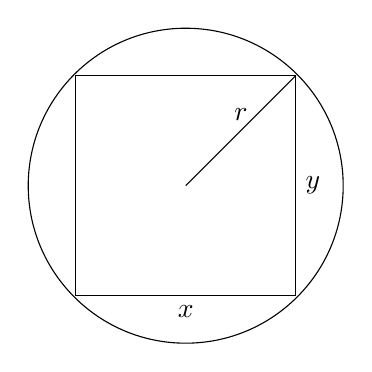
\begin{tikzpicture}
      \draw (0,0) circle (2cm);
      \draw (0,0) -- (0.701,0.701) node[above,fill=none] {$r$} -- (1.40,1.40);
      \draw (1.40,1.40) -- (1.40, 0) node[right,fill=none] {$y$} -- (1.40,-1.40)
      -- (0,-1.40) node[below,fill=none] {$x$} -- (-1.40,-1.40) -- (-1.40,1.40)
      -- cycle;
    \end{tikzpicture}
    \end{center}
    From the above diagram we see that $y = \sqrt{4r^2-x^2}$ and the area of the
    square is
    \begin{align*}
      A &= xy \\
      &= x\sqrt{4r^2 - x^2}
    \end{align*}
    To find the critical points
    \begin{align*}
      &\frac{dA}{dx} = \sqrt{4r^2-x^2} - \dfrac{x^2}{\sqrt{4r^2-x^2}} = \\
      & \Rightarrow 4r^2 - x^2 - x^2 = 0 \\
      & x = \sqrt{2} r \Rightarrow y = \sqrt{2} r.
    \end{align*}
    The other critical point is $x = 2r$ and comes from when
    $\dfrac{dA}{dx}$ is undefined. However, this would result in $y=0$ which is
    not part of the problem domain. We must check that $x=\sqrt{2} r$ is indeed
    a maximum, so let's use the first derivative test
    \begin{center}
    \begin{tikzpicture}
      \draw[->] (0,0) node[above left,fill=none] {$\sfrac{dA}{dx}$} -- (2,0)
      node[above,fill=none] {$(+)$} -- (4,0) -- (6,0) node[above,fill=none]
      {$(-)$} -- (8,0) node[right,fill=none] {$x$};
      \draw (4,-0.1) node[below,fill=none] {$\sqrt{2} r$} -- (4,0.1)
      node[above,fill=none] {Max};
    \end{tikzpicture}
    \end{center}
    Therefore, since this is a max and $x=y$ we see that the largest rectangle
    inscribed in a circle is indeed a square.
\end{solution}

\begin{problem}[3.]
  Show that if $x,y,\text{ and } z$ are positive numbers then
  \begin{equation*}
    \dfrac{\left( x^2 + 1 \right)\left( y^2 + 1 \right)\left( z^2 + 1
    \right)}{xyz} \ge 8
  \end{equation*}
  Hint: If $A$ and $B$ are both minimal then so is $AB$.
\end{problem}

\begin{solution}
  From the hint we see that if we minimize each of $f(x) = \dfrac{x^2+1}{x},\,
  g(y)=\dfrac{y^2+1}{y}, \text{ and } h(z)=\dfrac{z^2+1}{z}$ then we have minimized the
  product. Additionally, since the only difference between each of these is the
  variable the minimum is the same for each, so we only need to find the minimum
  of one of them. Let's find the minimum of $f(x)=\dfrac{x^2+1}{x}$.
  \begin{align*}
    f'(x) &= 1 - \frac{1}{x^2} = 0 \\
    \Rightarrow & x^2 - 1 = 0 \\
    & x = \pm 1
  \end{align*}
  The other critical point is $x=0$, because $f'(x)$ is undefined. However, the
  original function is also undefined at this point, so it is not in our domain
  and can be ignored. Additionally, the critical point $x=-1$ is not in our
  domain and can also be ignored. To determine which critical point is a min/max
  we will use the second derivative test
  \begin{equation*}
    f''(1) &= \frac{2}{(1)^3} > 0 \Rightarrow \text{Min}
  \end{equation*}
  This is indeed a minimum and the value is $f(1) = 2$. Now using the hint we
  see that 
  \begin{equation*}
    \dfrac{(x^2+1)(y^2+1)(z^2+1)}{xyz} \ge 2\cdot 2\cdot 2 = 8.
  \end{equation*}
\end{solution}

\end{document}
